\section{Hiện thực giao diện người dùng (Frontend)}

\subsection{Công nghệ và kiến trúc giao diện}
Giao diện người dùng của nền tảng UniConnect được xây dựng theo mô hình ứng dụng đơn trang (Single Page Application - SPA) hiện đại, đáp ứng các tiêu chuẩn về tính tương tác thời gian thực, độ mượt mà và khả năng thích ứng đa nền tảng (Responsive Web Design).

Các công nghệ và thư viện chủ chốt được ứng dụng trong phân hệ Frontend bao gồm:
\begin{itemize}
    \item \textbf{Thư viện lõi React 18 kết hợp TypeScript:} Tận dụng tính năng Concurrent Rendering, phân tách mã theo cấu trúc Component hóa tái sử dụng cao, đảm bảo tính chặt chẽ về mặt kiểu dữ liệu và giảm thiểu tối đa các lỗi lúc thực thi (runtime errors).
    \item \textbf{Công cụ đóng gói Vite:} Cung cấp môi trường phát triển với tốc độ biên dịch cực nhanh dựa trên ES Modules nguyên bản (Native ESM), tối ưu hóa kích thước gói phát hành (bundle size) và hỗ trợ cơ chế tải động theo trang (Lazy Loading kết hợp React Suspense).
    \item \textbf{Kiến trúc điều hướng và Quản lý trạng thái:} Sử dụng \texttt{react-router-dom} (v6) để thiết lập luồng điều hướng SPA mượt mà không cần tải lại trang. Trạng thái xác thực phiên làm việc của người dùng (Authentication Context) và hệ thống thông báo trạng thái tức thời (Toast Notification Context) được quản lý tập trung thông qua React Context API.
    \item \textbf{Giao tiếp mạng bất đồng bộ:} Thư viện Axios được cấu hình với các Interceptor tự động gắn Access Token (Bearer JWT) vào tiêu đề mọi yêu cầu và chủ động xử lý các mã lỗi HTTP chuẩn mực (401 Unauthorized, 403 Forbidden, 422 Validation Error).
    \item \textbf{Thiết kế giao diện hiện đại (Styling \& Design System):} Kết hợp các biến CSS Tokens toàn cục cùng hệ thống lưới linh hoạt (Flexbox và CSS Grid), mang lại khả năng hiển thị đồng nhất, hỗ trợ tốt chế độ sáng/tối (Dark Mode) và thân thiện với thiết bị di động (Mobile-first).
    \item \textbf{Bộ biểu tượng Lucide Icons \& Xử lý Markdown:} Tích hợp bộ icon vector chuẩn hóa đồng bộ nhận diện trực quan cùng thư viện \texttt{react-markdown} kết hợp \texttt{remark-gfm} để hiển thị nội dung định dạng phong phú từ các bài đăng và câu trả lời thông minh của Trợ lý AI.
\end{itemize}

\subsection{Chi tiết các màn hình chức năng cốt lõi}
Dưới đây là chi tiết các màn hình chức năng tiêu biểu đã được hiện thực hóa và vận hành ổn định trên hệ thống:

\subsubsection{Màn hình Bảng điều khiển và Khám phá Hoạt động (Student Dashboard)}
Giao diện trung tâm cho phép sinh viên theo dõi toàn bộ các sự kiện học đường và phong trào tình nguyện sắp diễn ra. Hệ thống cung cấp bộ lọc đa tiêu chí (học thuật, thể thao, tình nguyện, CTXH), thanh tìm kiếm thông minh và các thẻ hoạt động trực quan hiển thị đầy đủ thông tin thời gian, địa điểm cũng như số ngày CTXH tích lũy.

\begin{figure}[H]
    \centering
    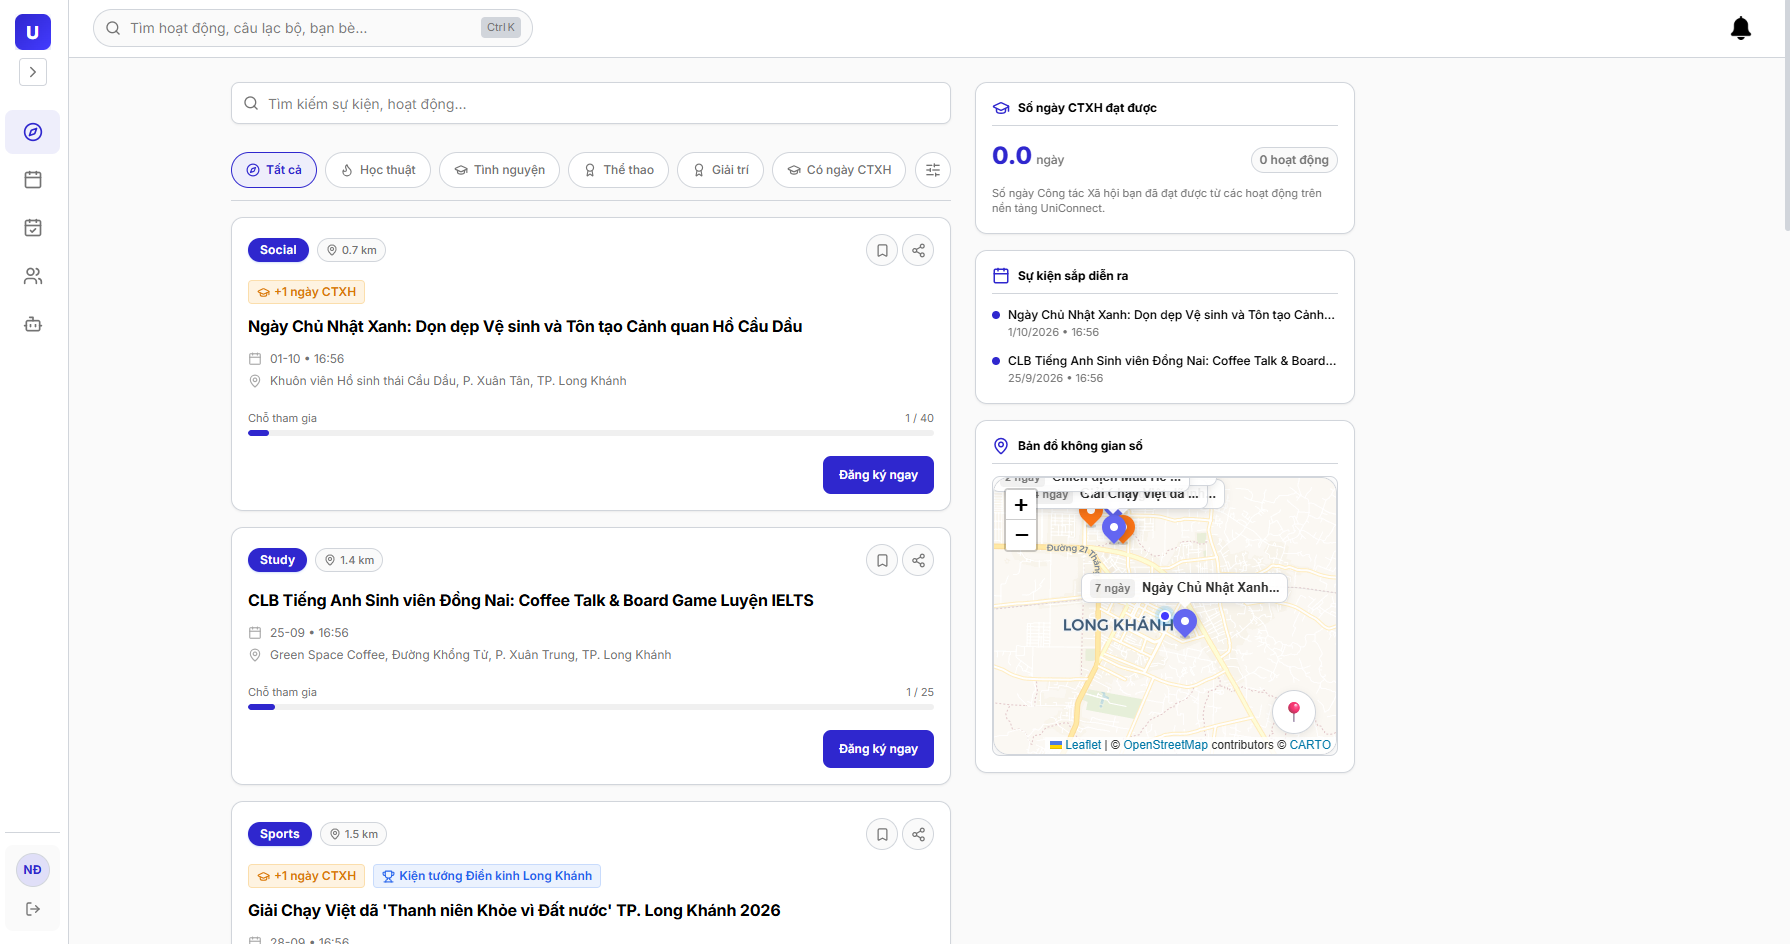
\includegraphics[width=0.68\textwidth]{Images/ui-dashboard.png}
    \caption{Giao diện Bảng điều khiển sinh viên và khám phá các hoạt động ngoại khóa}
    \label{fig:ui_dashboard}
\end{figure}

\subsubsection{Màn hình Chi tiết Hoạt động và Đăng ký tham gia (Activity Details)}
Cung cấp đầy đủ thông tin chi tiết về sự kiện: thời gian diễn ra, địa điểm tập trung, câu lạc bộ hoặc đơn vị tổ chức, số lượng suất tham gia còn lại và danh sách sinh viên tham dự. Hệ thống tự động đối soát lịch trình cá nhân theo thời gian thực để cảnh báo khả năng xung đột thời gian và cung cấp nút đăng ký tham gia trực tiếp.

\begin{figure}[H]
    \centering
    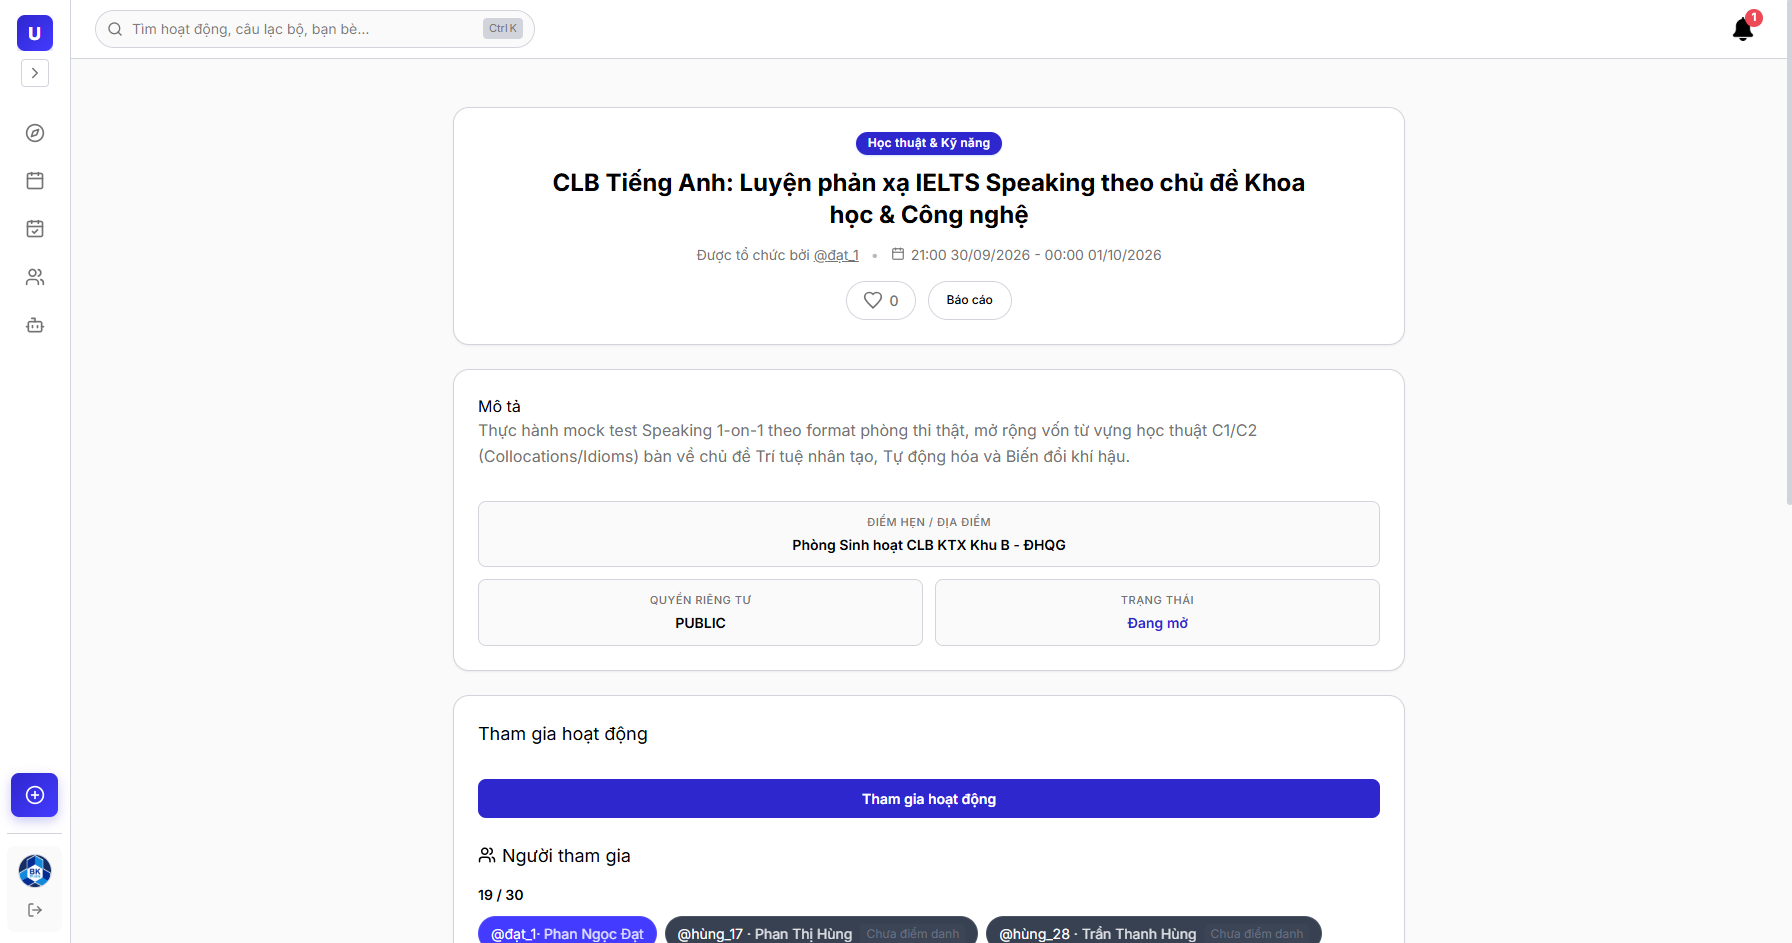
\includegraphics[width=0.68\textwidth]{Images/ui-activity-detail.png}
    \caption{Giao diện Chi tiết hoạt động và đối soát lịch trình đăng ký}
    \label{fig:ui_activity_detail}
\end{figure}

\clearpage
\subsubsection{Màn hình Khởi tạo và Thiết lập Hoạt động (Create Activity)}
Giao diện dành cho ban tổ chức và ban chủ nhiệm các câu lạc bộ để thiết lập sự kiện mới. Biểu mẫu hỗ trợ cấu hình toàn diện các thông số: tiêu đề, mô tả chi tiết, danh mục, thời gian diễn ra, địa điểm tổ chức trên bản đồ, số lượng người tham gia tối đa, định mức ngày CTXH và tùy chọn phê duyệt đơn tham gia.

\begin{figure}[H]
    \centering
    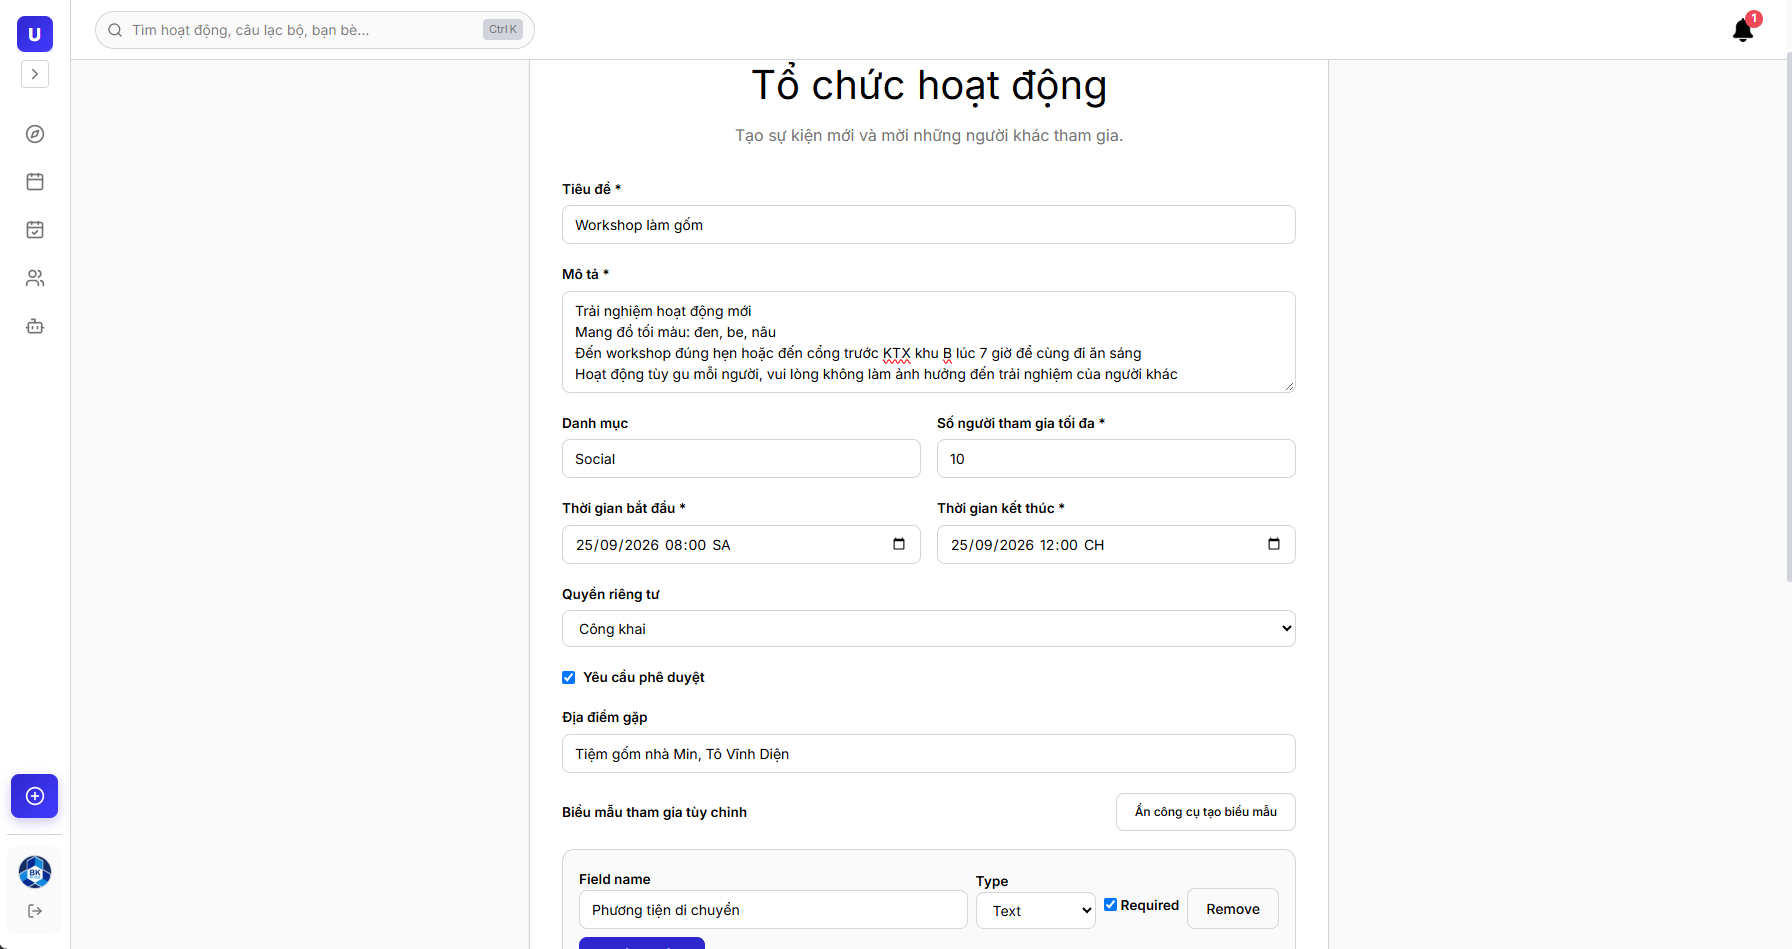
\includegraphics[width=0.68\textwidth]{Images/ui-tao-hoat-dong.png}
    \caption{Giao diện Khởi tạo và thiết lập thông số hoạt động phong trào mới}
    \label{fig:ui_tao_hoat_dong}
\end{figure}

\subsubsection{Màn hình Lịch Thông minh và Quản lý Lịch trình (Smart Calendar Schedule)}
Hiển thị trực quan lịch trình cá nhân của sinh viên theo các chế độ xem linh hoạt (tuần/tháng), tích hợp đồng thời các khung giờ bận cố định (thời khóa biểu học tập) cùng các sự kiện ngoại khóa đã xác nhận tham gia. Hệ thống hỗ trợ chức năng xuất nhanh tệp chuẩn \texttt{.ics} để đồng bộ lịch trình hai chiều vào Google Calendar hoặc Apple Calendar.

\begin{figure}[H]
    \centering
    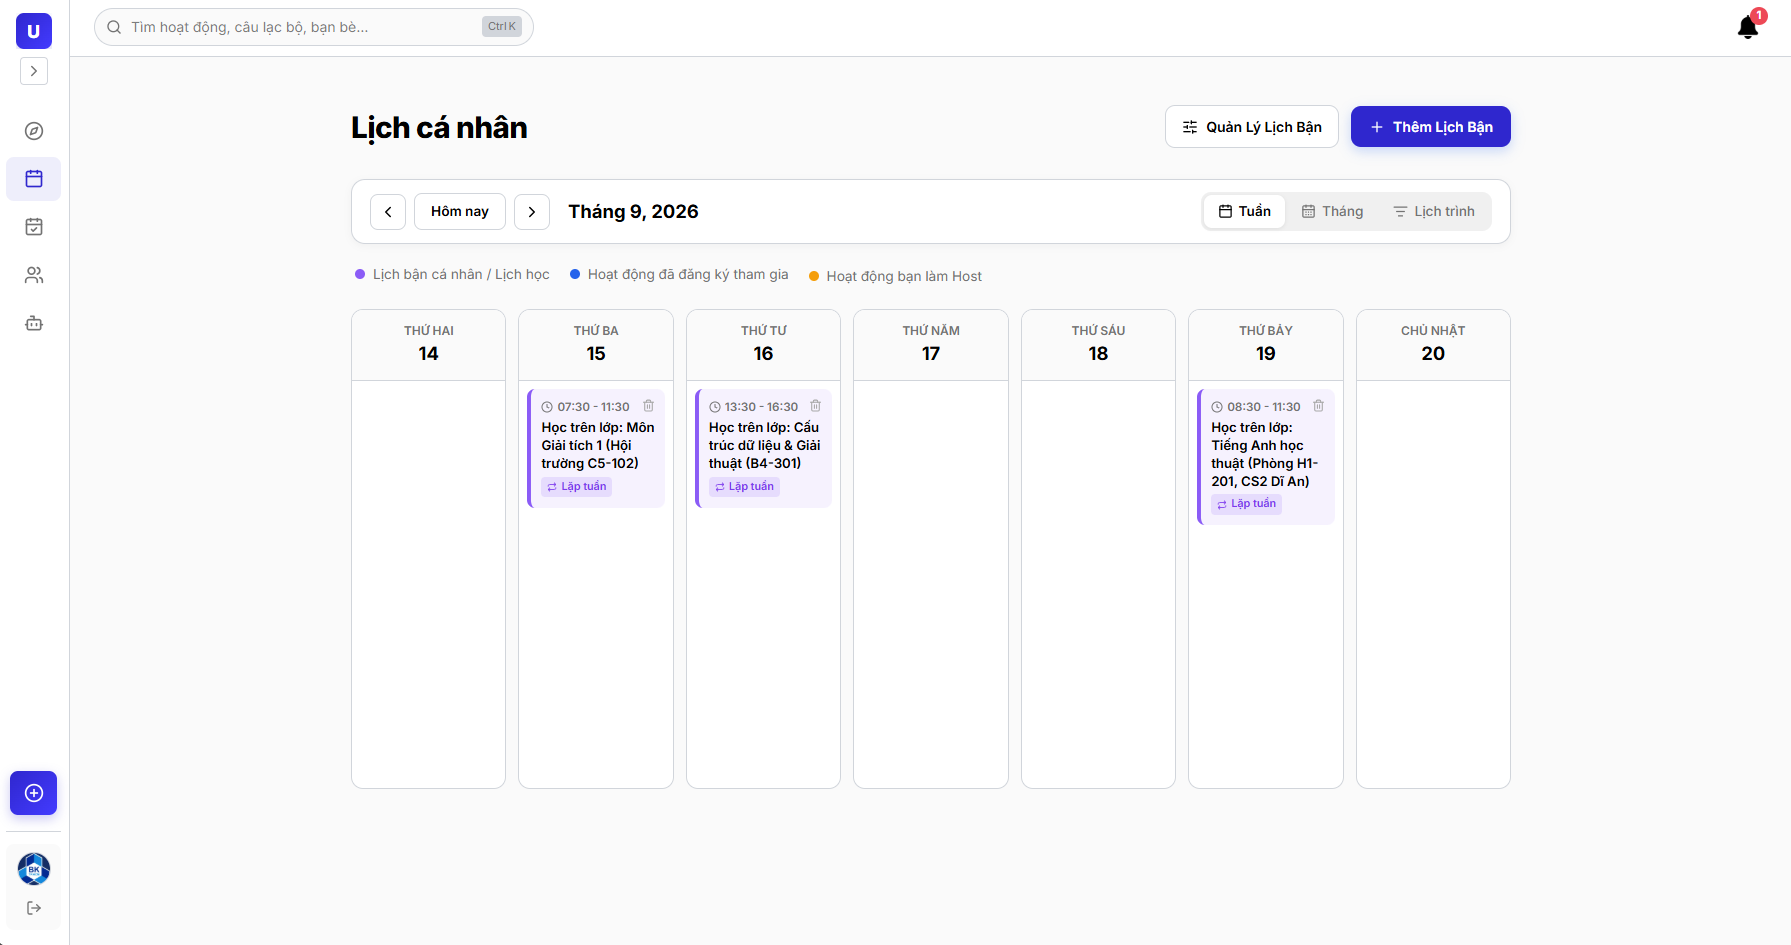
\includegraphics[width=0.68\textwidth]{Images/ui-lich-ca-nhan.png}
    \caption{Giao diện Lịch thông minh và quản lý khung giờ bận cá nhân}
    \label{fig:ui_smart_calendar}
\end{figure}

\clearpage
\subsubsection{Màn hình Trợ lý Học đường AI Thông minh (AI Assistant Chatbot)}
Giao diện tương tác trò chuyện với Trợ lý AI UniConnect. Người dùng có thể đặt câu hỏi tự nhiên để nhờ tìm kiếm sự kiện phù hợp, đối soát lịch bận cá nhân hoặc tra cứu các câu lạc bộ học đường. Phản hồi của Trợ lý AI cung cấp đầy đủ thông tin súc tích kèm theo các đường dẫn (hyperlink) điều hướng trực tiếp đến trang chi tiết hoạt động và câu lạc bộ tương ứng.

\begin{figure}[H]
    \centering
    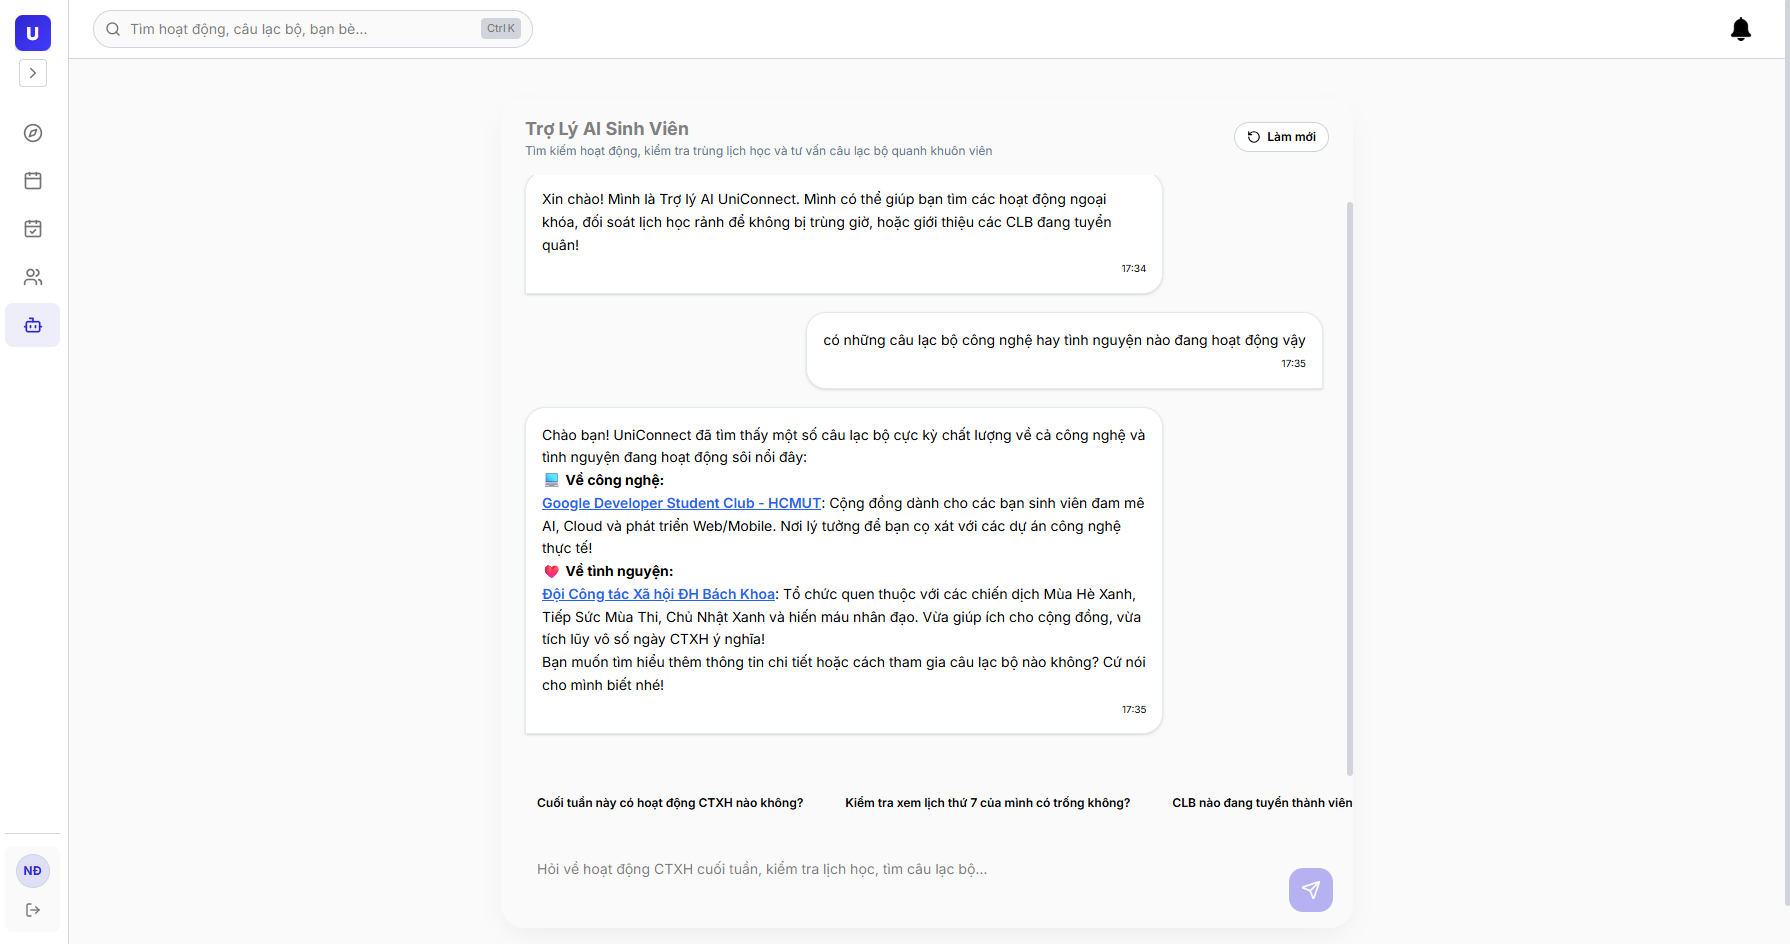
\includegraphics[width=0.68\textwidth]{Images/ui-chatbot.png}
    \caption{Giao diện Trợ lý học đường AI giải đáp thông tin và gợi ý hoạt động}
    \label{fig:ui_chatbot}
\end{figure}

\subsubsection{Màn hình Cộng đồng và Câu lạc bộ Sinh viên (Student Communities \& Clubs)}
Không gian kết nối và sinh hoạt của các câu lạc bộ, đội nhóm phong trào trong toàn trường. Người dùng có thể tra cứu thông tin giới thiệu, mục tiêu hoạt động, số lượng thành viên của từng CLB và nộp đơn đăng ký tham gia cộng đồng.

\begin{figure}[H]
    \centering
    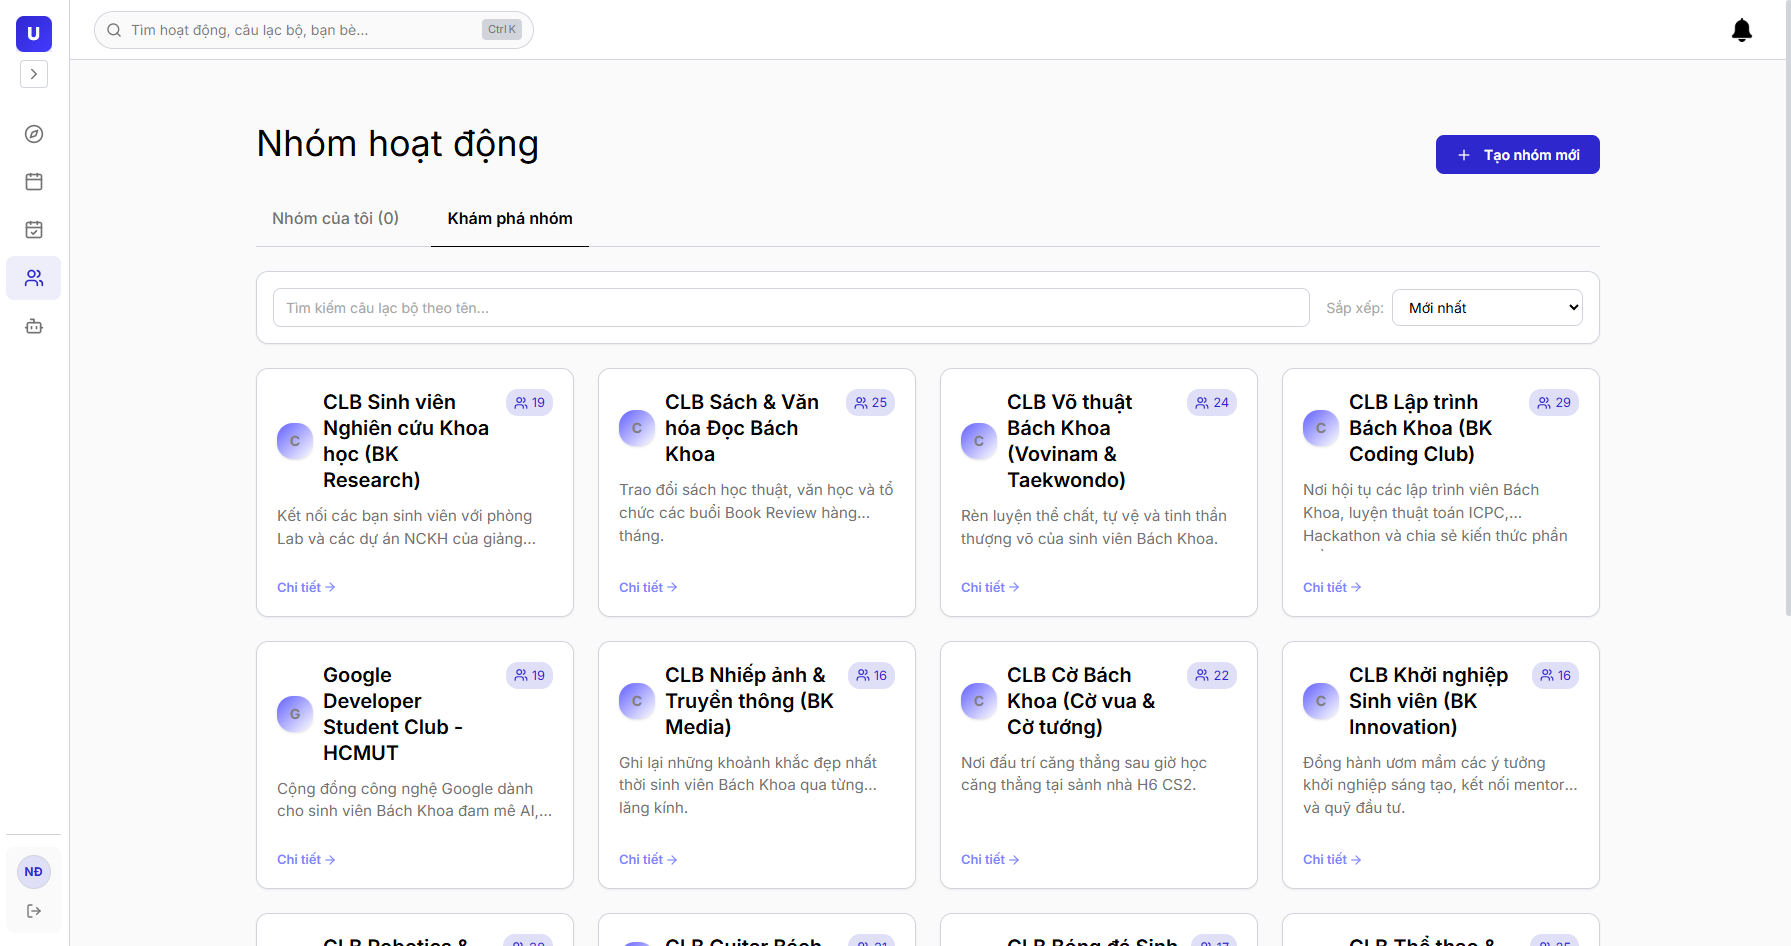
\includegraphics[width=0.68\textwidth]{Images/ui-nhom.png}
    \caption{Giao diện Danh sách và thông tin các câu lạc bộ, đội nhóm học đường}
    \label{fig:ui_nhom}
\end{figure}

\clearpage
\subsubsection{Màn hình Hồ sơ Cá nhân và Vinh danh Thành tích (Gamification Profile)}
Không gian vinh danh nỗ lực tham gia hoạt động của sinh viên: hiển thị tổng số ngày Công tác Xã hội (CTXH) tích lũy, cấp bậc thứ hạng sinh viên, tủ trưng bày bộ sưu tập danh hiệu Trophy đã mở khóa và lịch sử chi tiết các sự kiện sinh viên đã tham gia.

\begin{figure}[H]
    \centering
    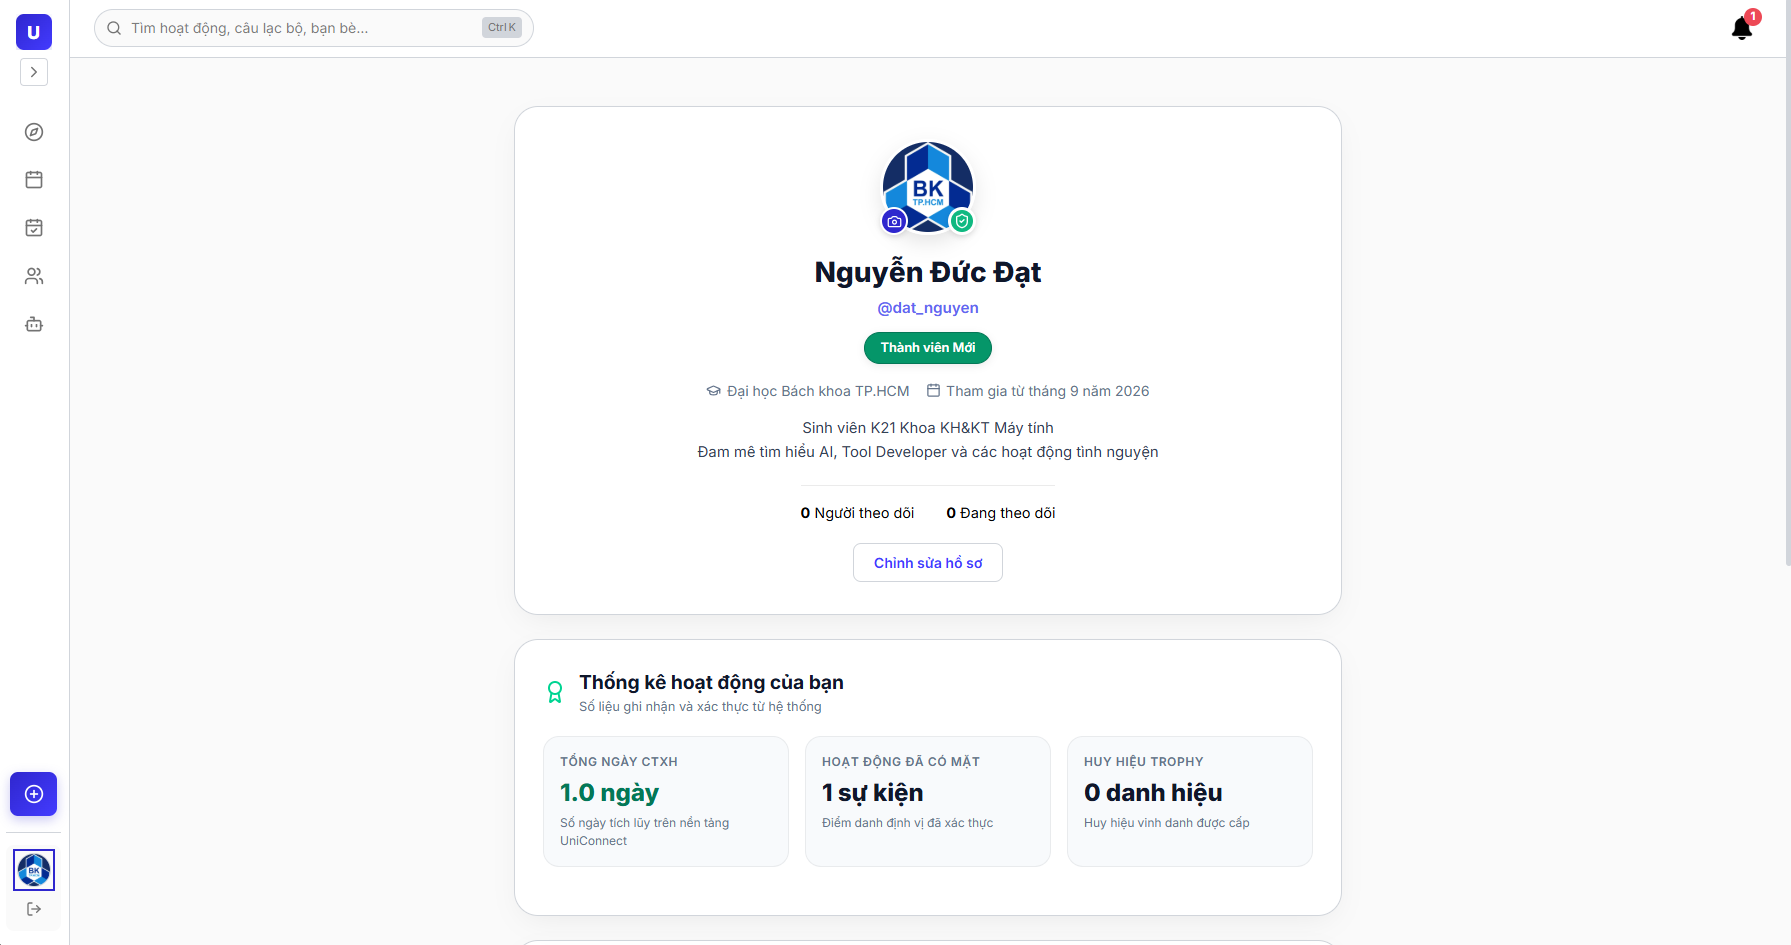
\includegraphics[width=0.68\textwidth]{Images/ui-profile.png}
    \caption{Giao diện Hồ sơ cá nhân, tiến trình tích lũy CTXH và danh hiệu Trophy}
    \label{fig:ui_profile}
\end{figure}

\subsubsection{Màn hình Giấy xác nhận Tham gia Hoạt động (Activity Participation Certificate)}
Biểu mẫu hành chính điện tử công nhận sự tham gia của sinh viên sau khi hoàn thành hoạt động. Giấy xác nhận được trình bày theo thể thức văn bản chuẩn mực, bao gồm tên đơn vị tổ chức, tên hoạt động, số ngày CTXH ghi nhận, mã tra cứu xác thực và nút tải trực tiếp tệp tin PDF về máy phục vụ cho việc nộp minh chứng điểm rèn luyện.

\begin{figure}[H]
    \centering
    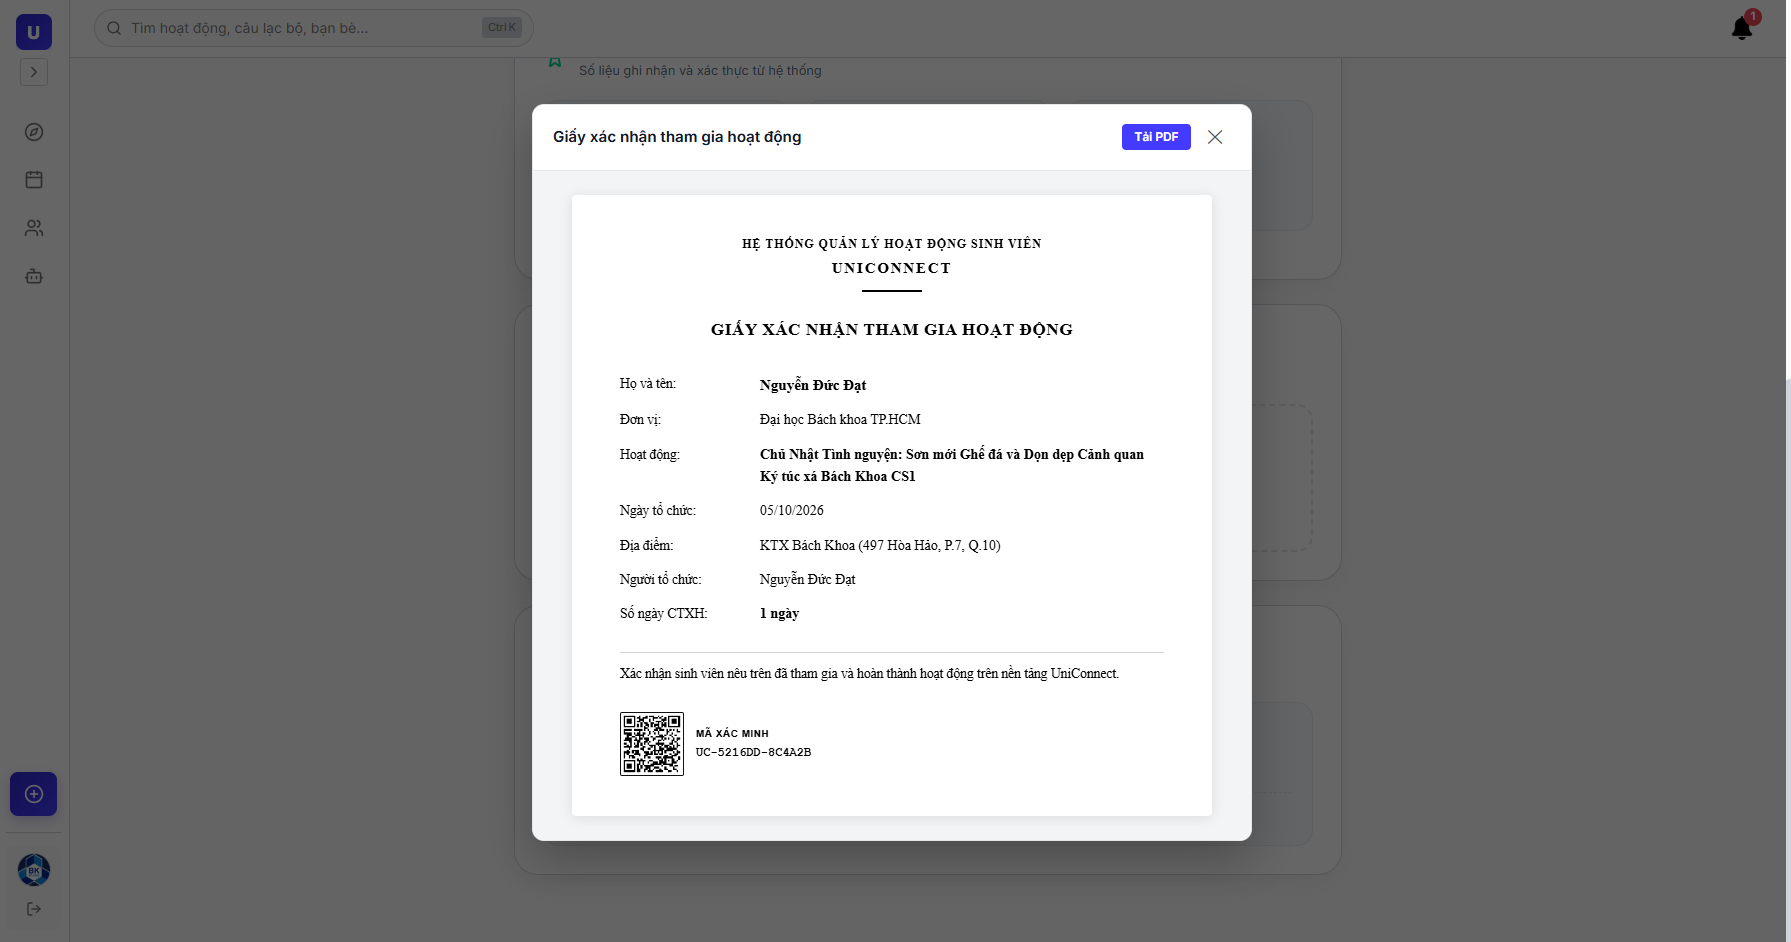
\includegraphics[width=0.68\textwidth]{Images/ui-giay-xac-nhan-tham-gia.png}
    \caption{Giao diện Giấy xác nhận tham gia hoạt động điện tử chuẩn hành chính}
    \label{fig:ui_certificate_modal}
\end{figure}

\subsection{Kết luận chương}
Chương này đã trình bày toàn diện quá trình hiện thực hóa giao diện người dùng Frontend của nền tảng UniConnect. Bằng việc ứng dụng React 18, TypeScript, Vite và ngôn ngữ thiết kế chuẩn mực, hệ thống mang lại trải nghiệm tương tác trực quan, mượt mà và thích ứng linh hoạt đa thiết bị. Toàn bộ 8 màn hình chức năng cốt lõi đã được hoàn thiện chỉn chu, tối ưu hóa kích thước gói tải, bảo đảm tính toàn vẹn dữ liệu và sẵn sàng phục vụ nhu cầu phong trào thực tế của sinh viên.
